\section{Fonction $\frac{1-z^{-1}}{2}$}
Nous commençons par afficher le diagramme de gain en décibel (\ref{f1 Diagramme de gain}) ainsi que le diagramme de phase en radians (\ref{f1 Diagramme de phase}) pour déterminer la nature du filtre représenté par cette fonction de transfert.
\begin{figure}[H]
\centering
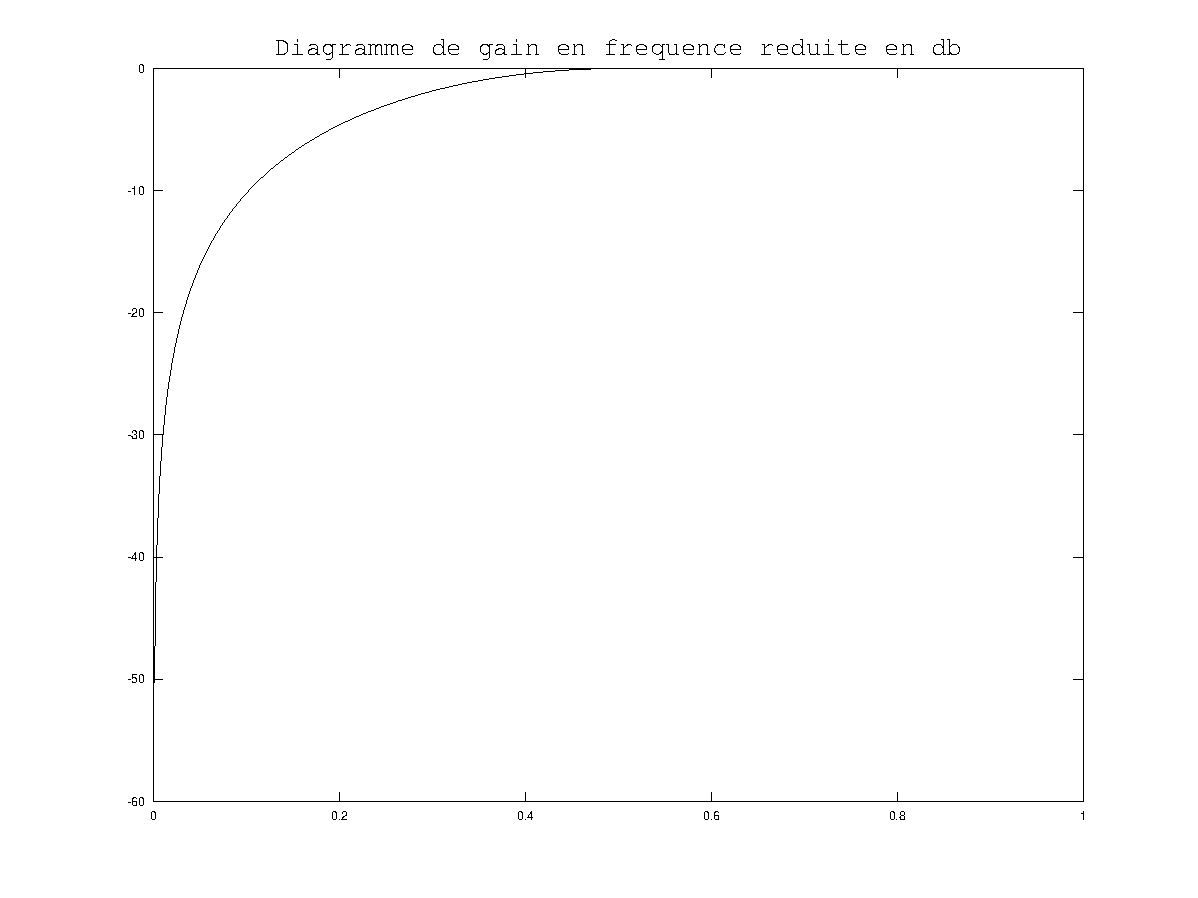
\includegraphics[width=9cm]{resEx3/f1Gain.pdf}
\caption{Diagramme de gain de la fonction $\frac{1-z^{-1}}{2}$ en dB}
\label{f1 Diagramme de gain}
\end{figure}
\begin{figure}[H]
\centering
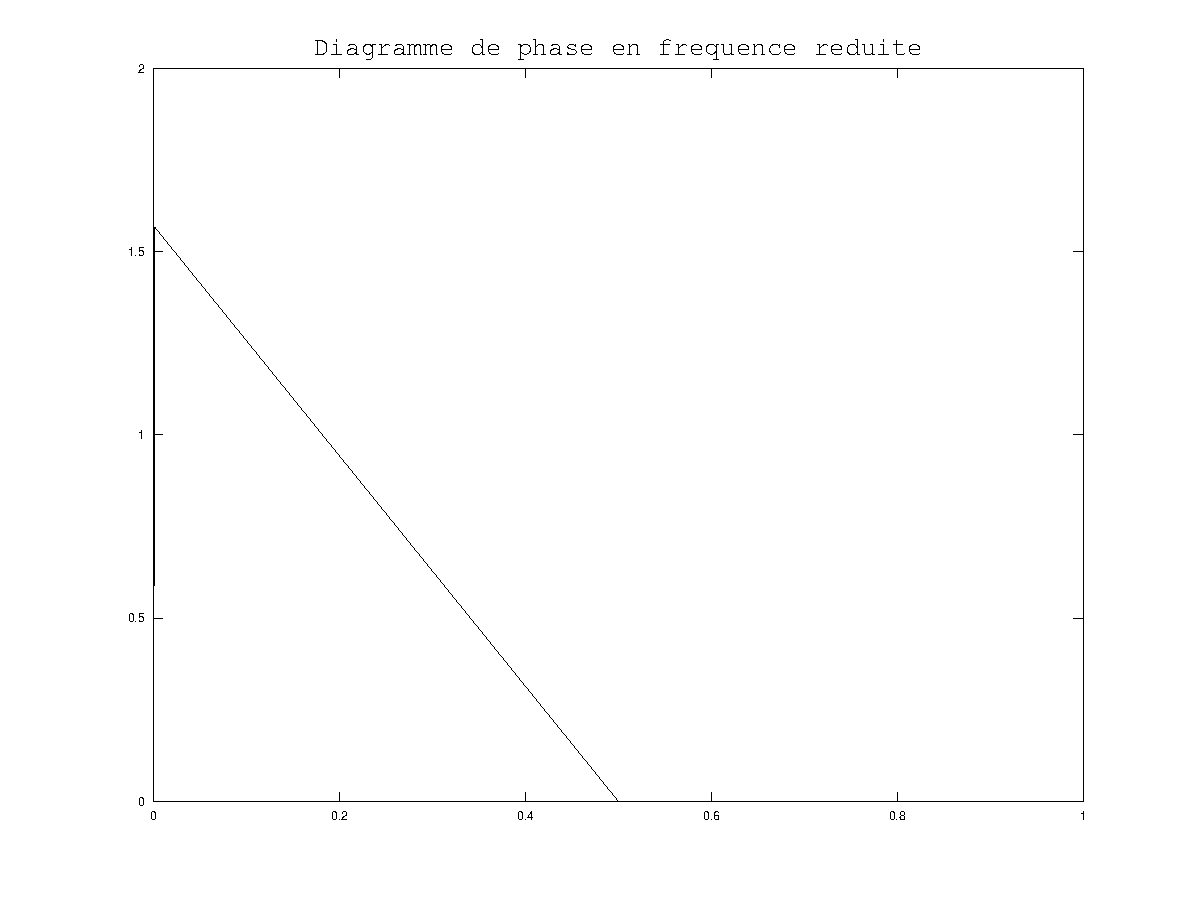
\includegraphics[width=9cm]{resEx3/f1Phase.pdf}
\caption{Diagramme de phase de la fonction $\frac{1-z^{-1}}{2}$ en radians}
\label{f1 Diagramme de phase}
\end{figure}
Nous pouvons donc constater que cette fonction de transfert en z correspond à un filtre passe haut.
\subsection{Réponse impulsionnelle}
~\\
\begin{figure}[H]
\centering
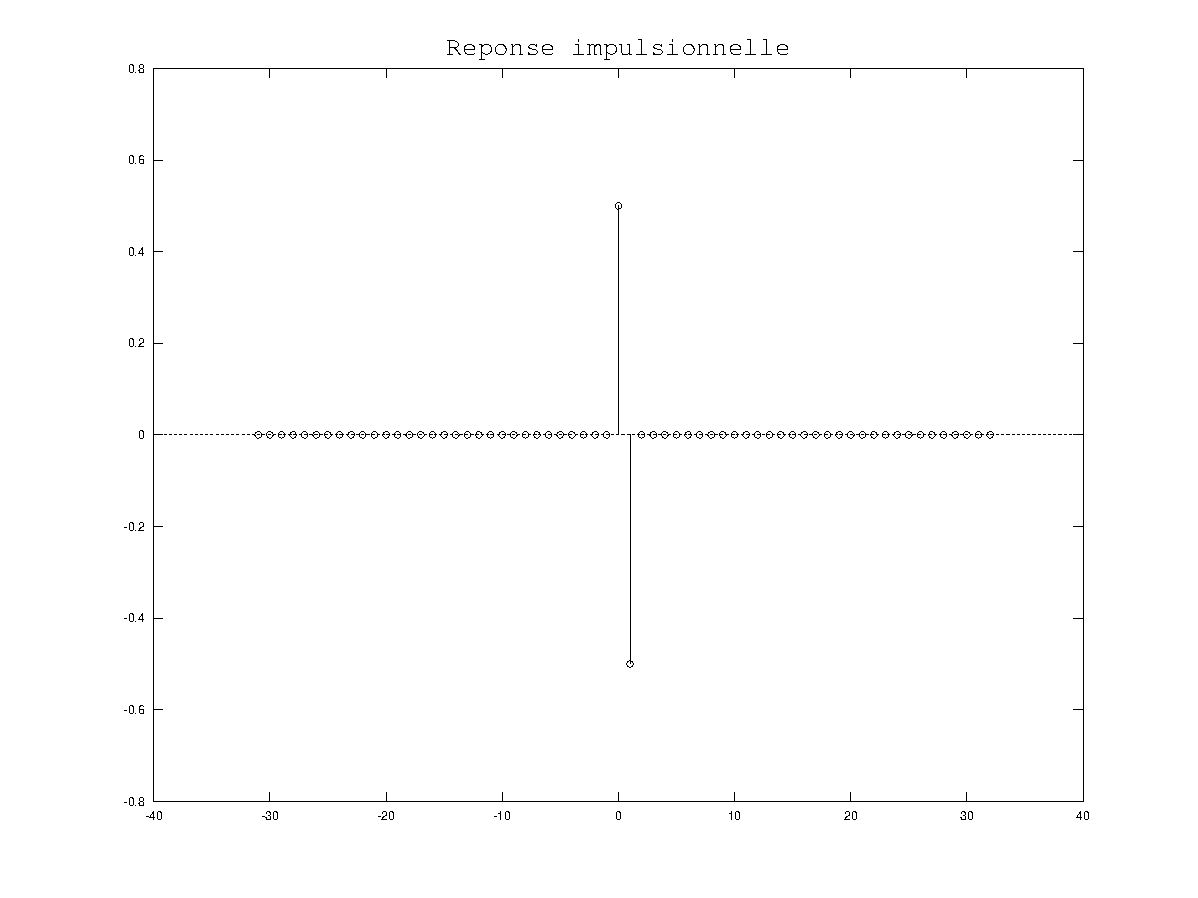
\includegraphics[width=9cm]{resEx3/f1Impulsion.pdf}
\caption{Réponse impulsionnelle de la fonction $\frac{1-z^{-1}}{2}$ }
\end{figure}
\subsection{Réponse indicielle}
~\\
\begin{figure}[H]
\centering
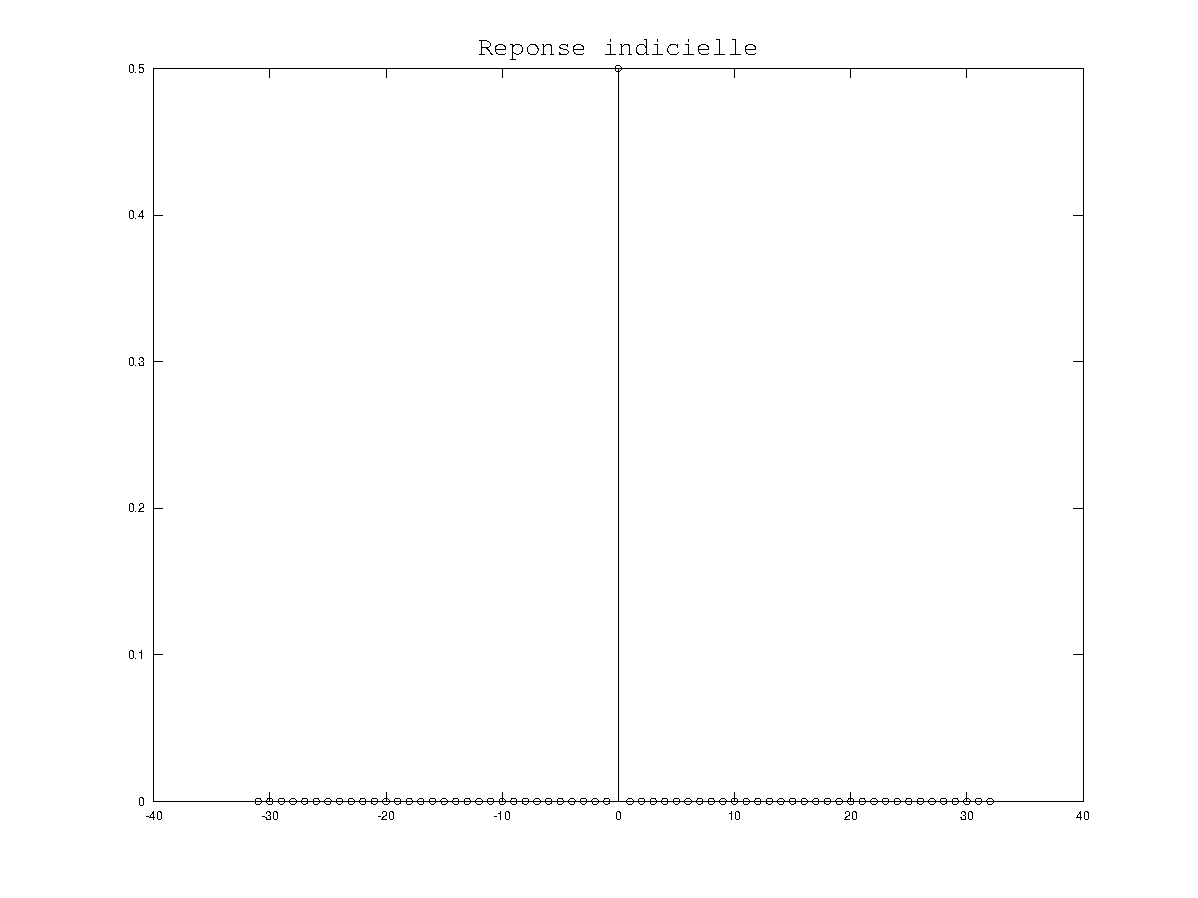
\includegraphics[width=9cm]{resEx3/f1Indice.pdf}
\caption{Réponse indicielle de la fonction $\frac{1-z^{-1}}{2}$ }
\end{figure}

\subsection{Les zéros et les pôles}
~\\
\begin{figure}[H]
\centering
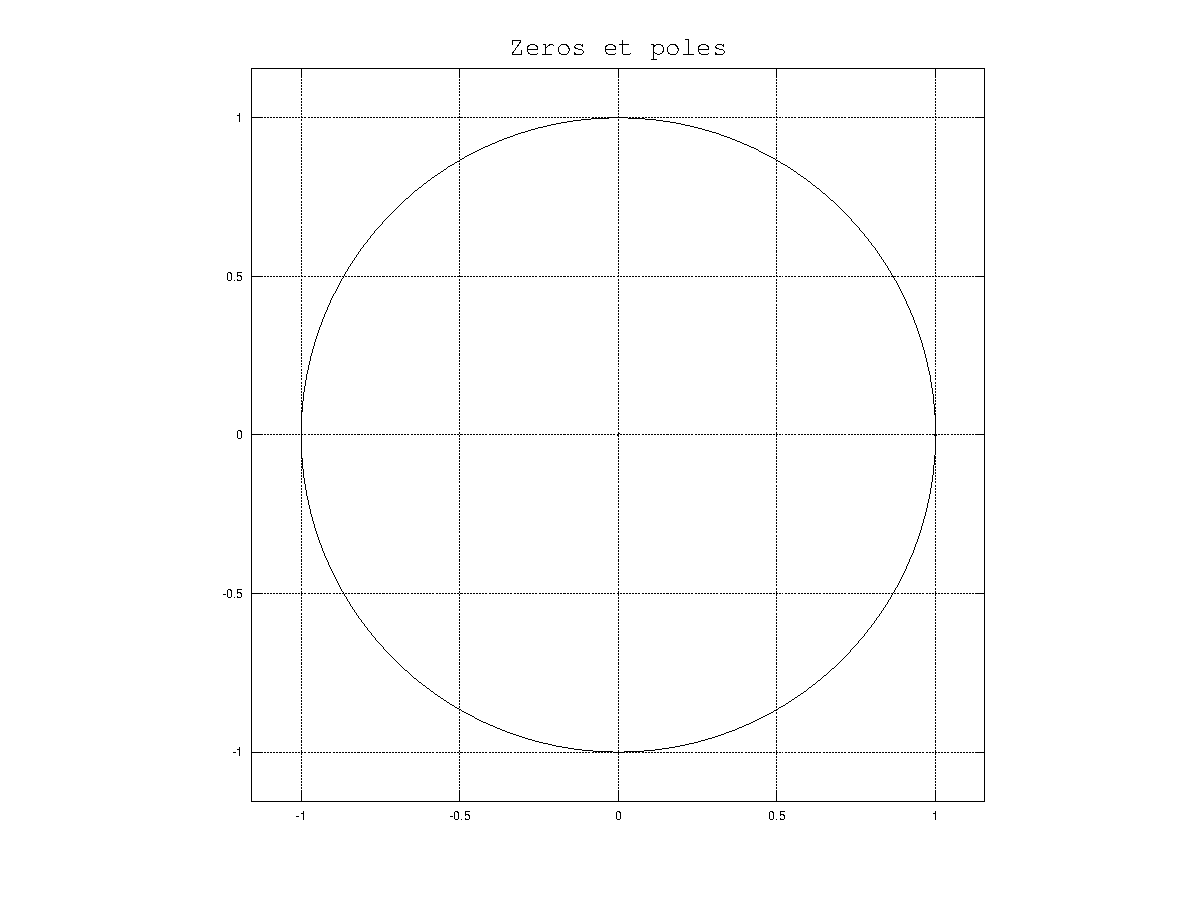
\includegraphics[width=9cm]{resEx3/f1ZP.pdf}
\caption{Les zéros et les pôles de la fonction $\frac{1-z^{-1}}{2}$ }
\end{figure}


\section{Fonction $\frac{1+z^{-1}}{2}$}
Nous commençons par afficher le diagramme de gain en décibel (\ref{f2 Diagramme de gain}) ainsi que le diagramme de phase en radians (\ref{f2 Diagramme de phase}) pour déterminer la nature du filtre représenté par cette fonction de transfert.
\begin{figure}[H]
\centering
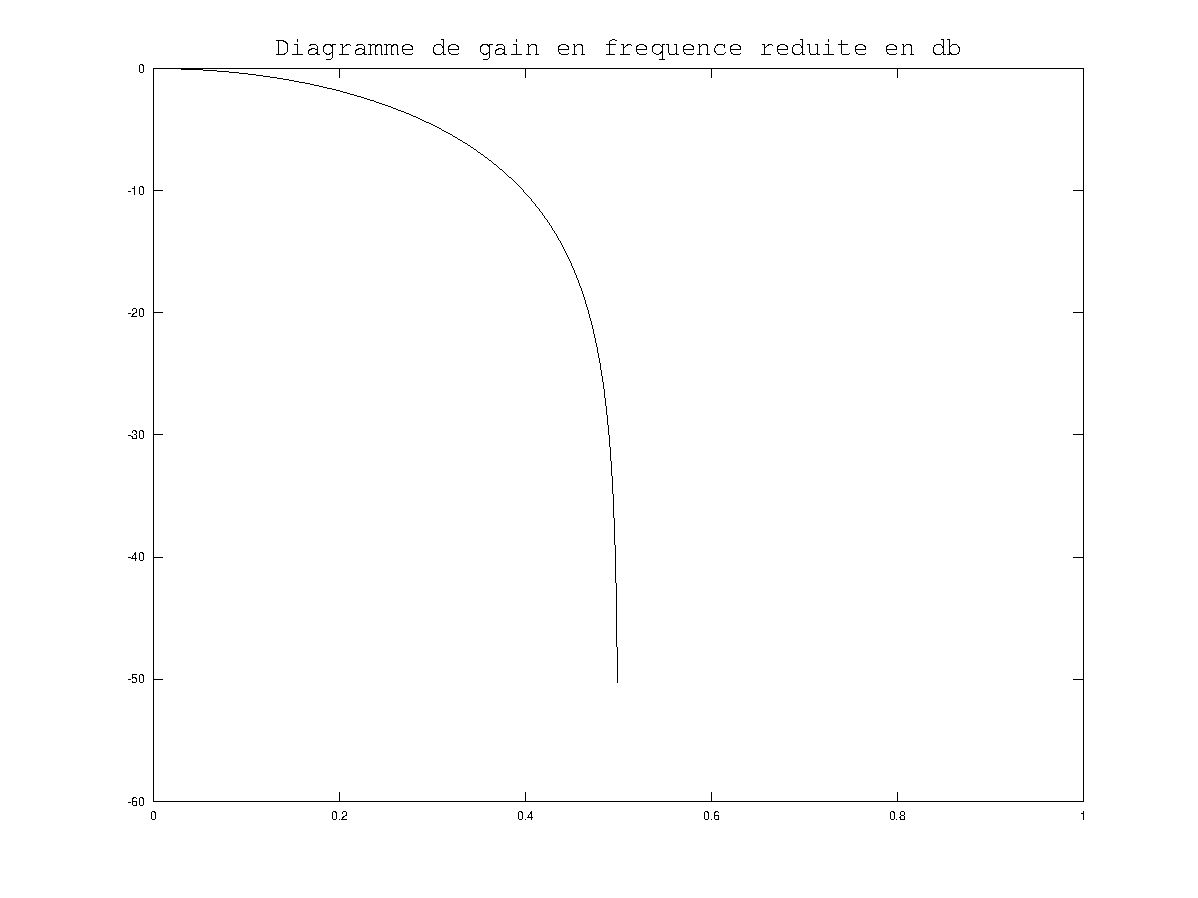
\includegraphics[width=9cm]{resEx3/f2Gain.pdf}
\caption{Diagramme de gain de la fonction $\frac{1+z^{-1}}{2}$ en dB}
\label{f2 Diagramme de gain}
\end{figure}
\begin{figure}[H]
\centering
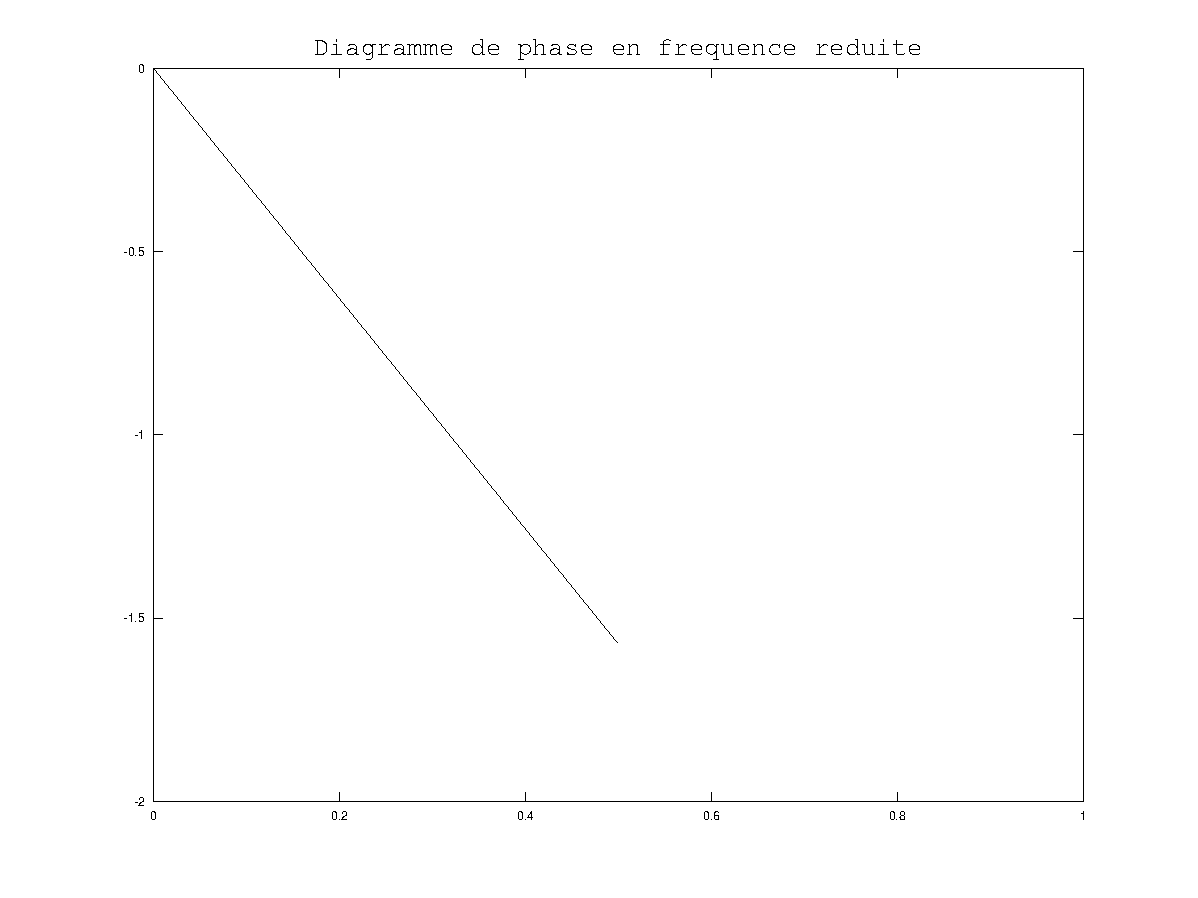
\includegraphics[width=9cm]{resEx3/f2Phase.pdf}
\caption{Diagramme de phase de la fonction $\frac{1+z^{-1}}{2}$ en radians}
\label{f2 Diagramme de phase}
\end{figure}
Nous pouvons donc constater que cette fonction de transfert en z correspond à un filtre passe bas.
\subsection{Réponse impulsionnelle}
~\\
\begin{figure}[H]
\centering
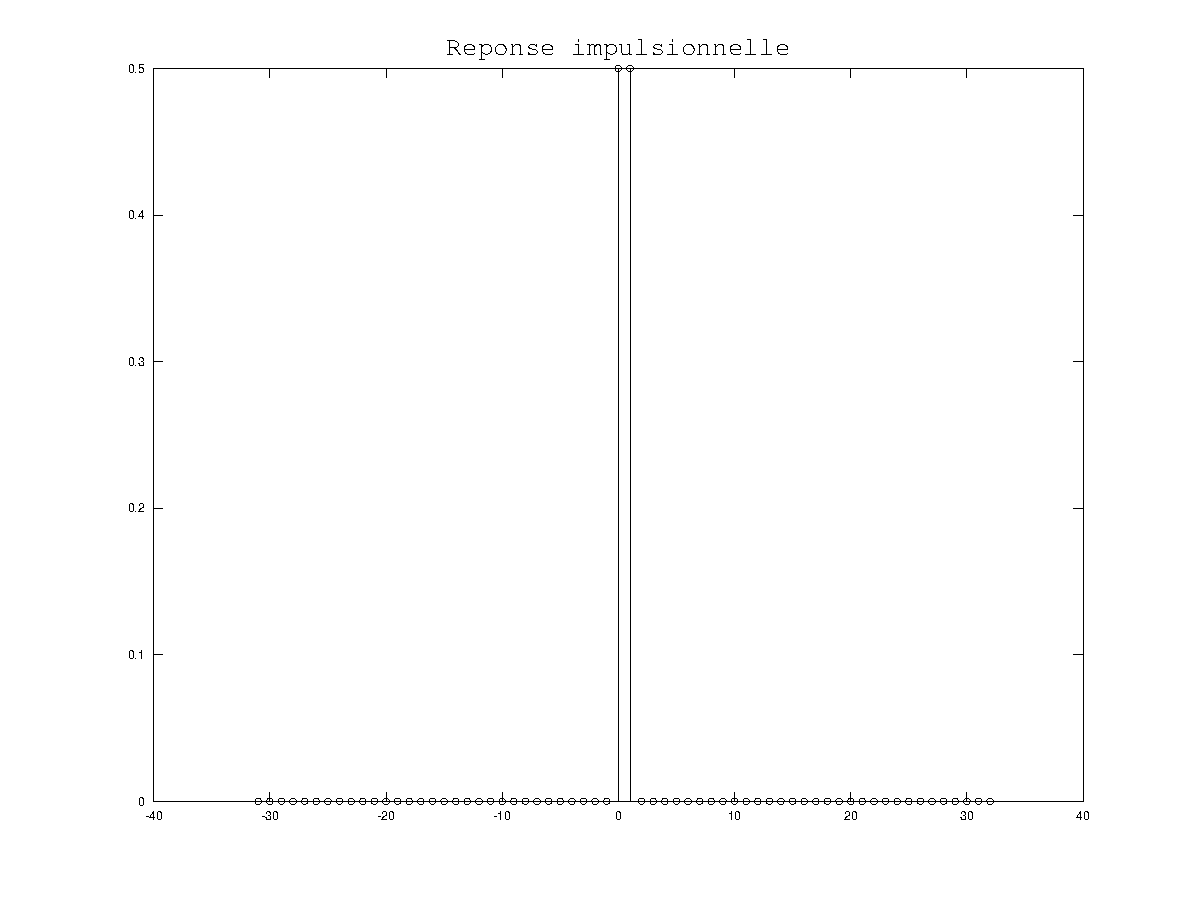
\includegraphics[width=9cm]{resEx3/f2Impulsion.pdf}
\caption{Réponse impulsionnelle de la fonction $\frac{1+z^{-1}}{2}$ }
\end{figure}

\subsection{Réponse indicielle}
~\\
\begin{figure}[H]
\centering
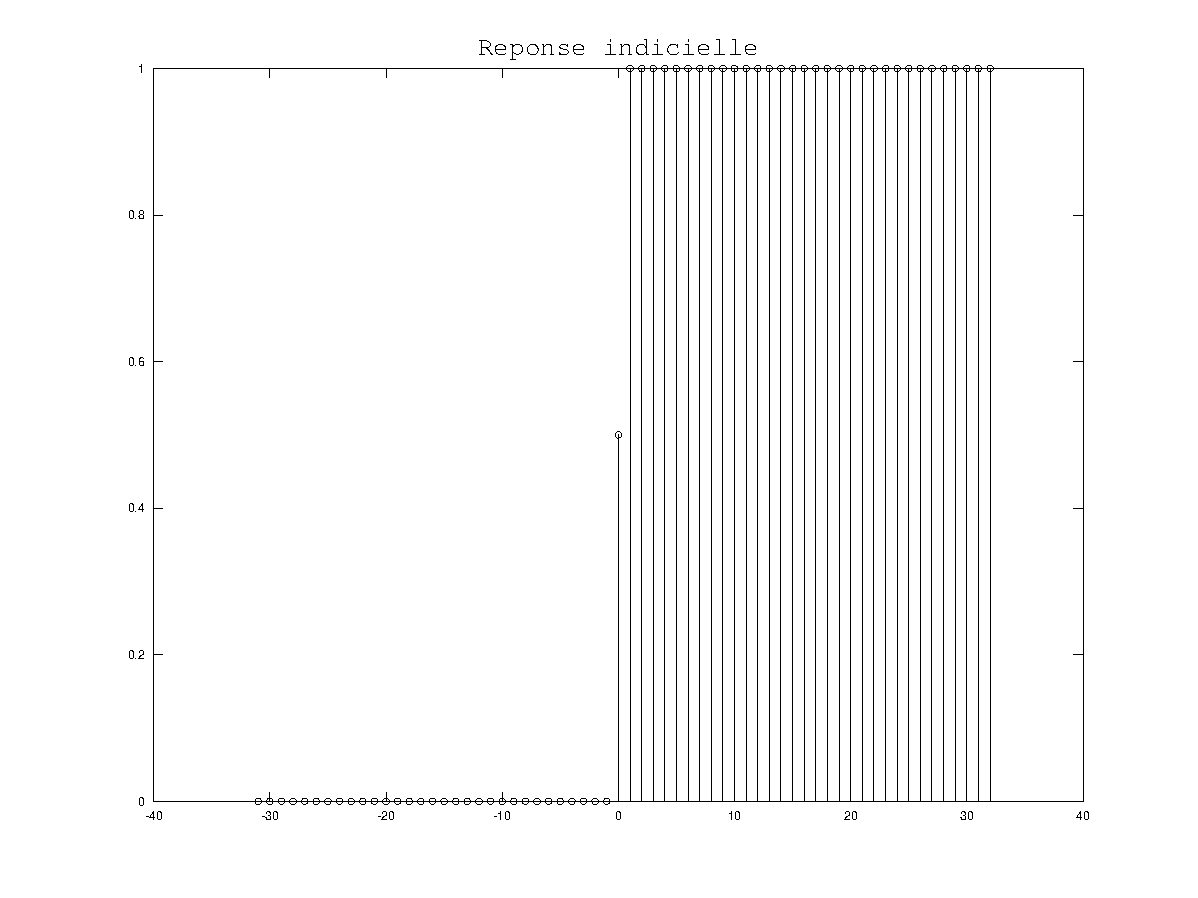
\includegraphics[width=9cm]{resEx3/f2Indice.pdf}
\caption{Réponse indicielle de la fonction $\frac{1+z^{-1}}{2}$ }
\end{figure}

\subsection{Les zéros et les pôles}
~\\
\begin{figure}[H]
\centering
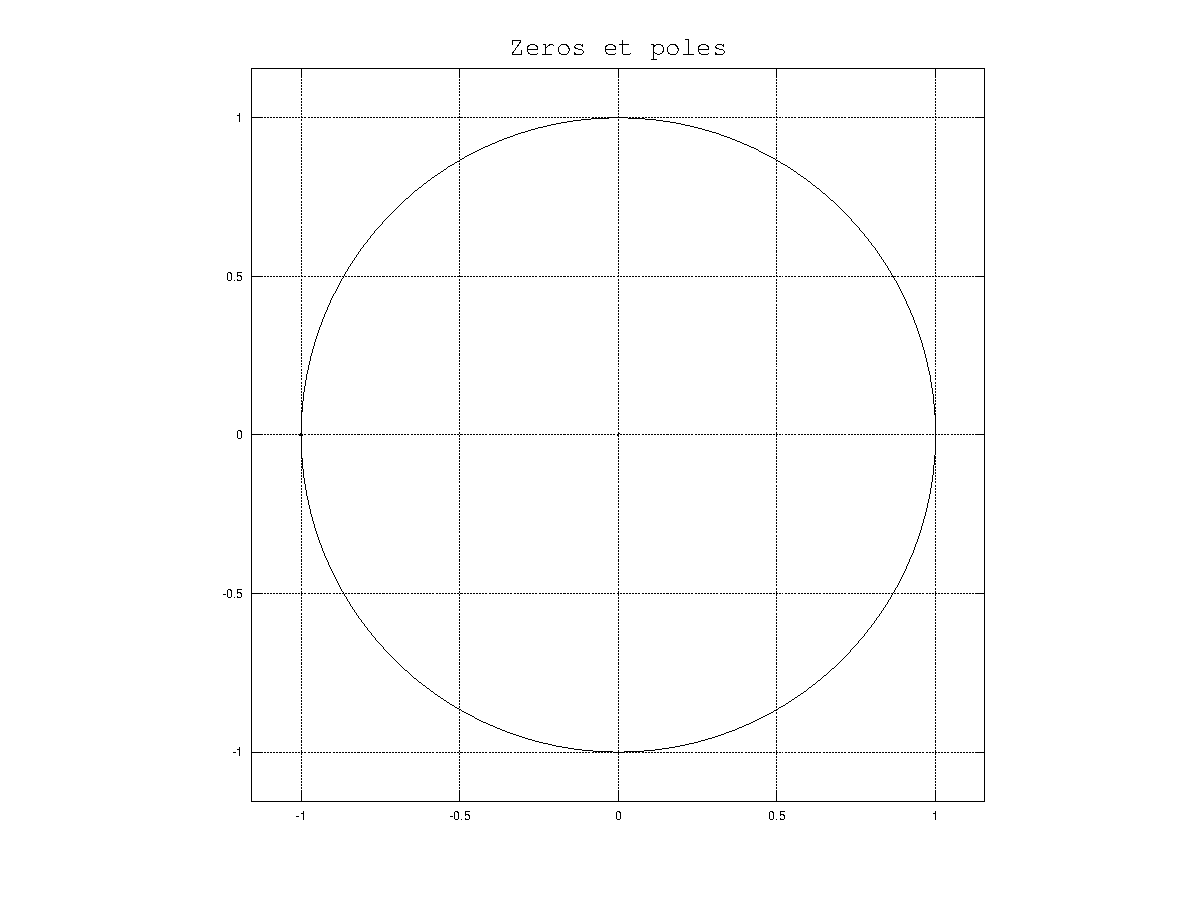
\includegraphics[width=9cm]{resEx3/f2ZP.pdf}
\caption{Les zéros et les pôles de la fonction $\frac{1+z^{-1}}{2}$ }
\end{figure}


\section{Fonction $\frac{1-z^{-2}}{2}$}
Nous commençons par afficher le diagramme de gain en décibel (\ref{f3 Diagramme de gain}) ainsi que le diagramme de phase en radians (\ref{f3 Diagramme de phase}) pour déterminer la nature du filtre représenté par cette fonction de transfert.
\begin{figure}[H]
\centering
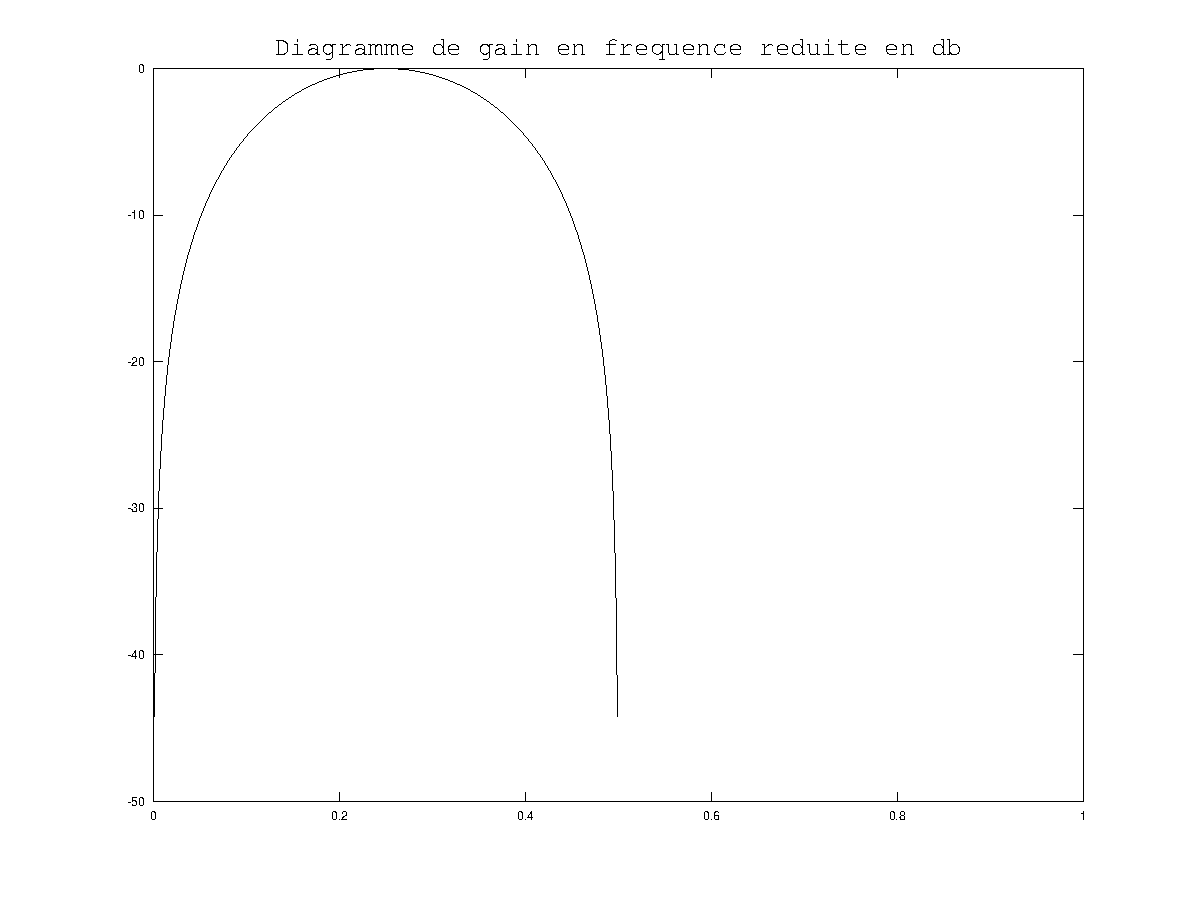
\includegraphics[width=9cm]{resEx3/f3Gain.pdf}
\caption{Diagramme de gain de la fonction $\frac{1-z^{-2}}{2}$ en dB}
\label{f3 Diagramme de gain}
\end{figure}
\begin{figure}[H]
\centering
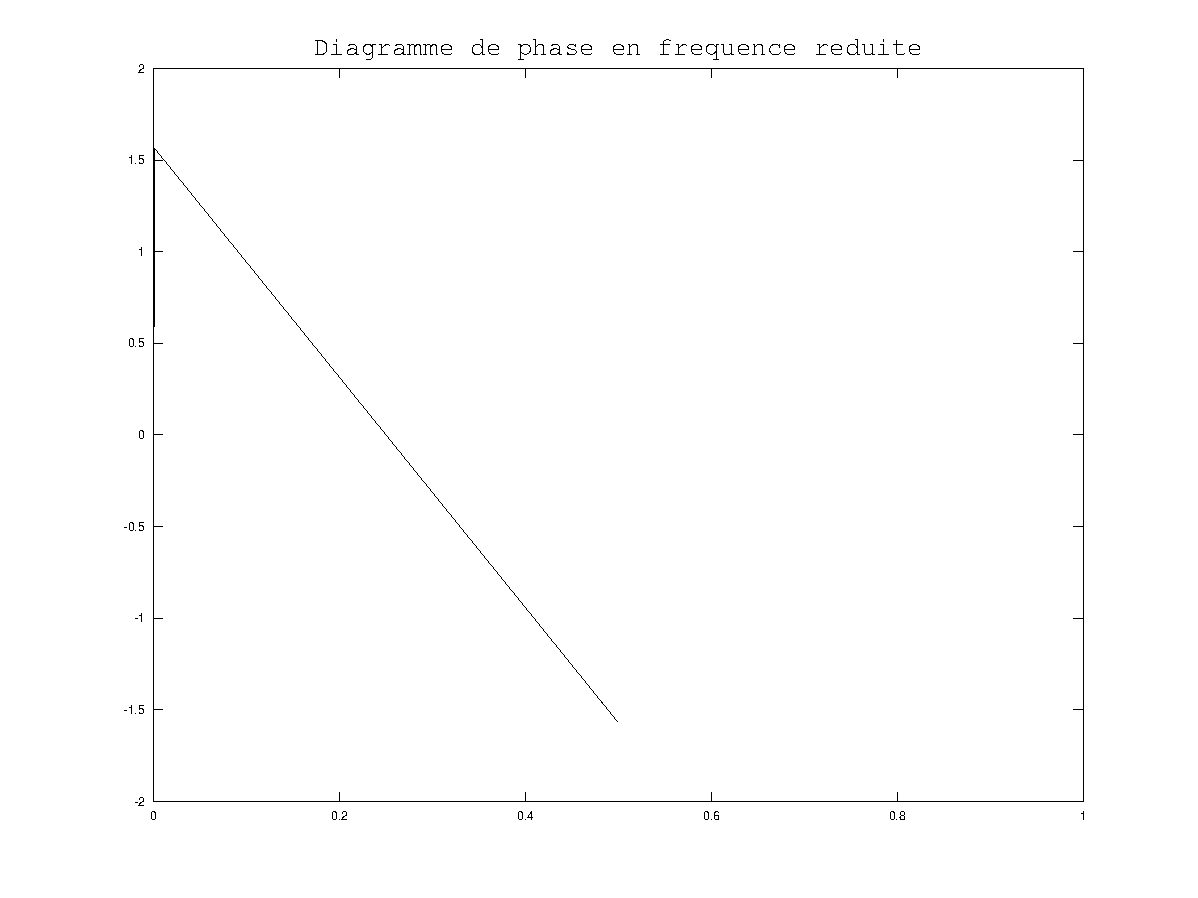
\includegraphics[width=9cm]{resEx3/f3Phase.pdf}
\caption{Diagramme de phase de la fonction $\frac{1-z^{-2}}{2}$ en radians}
\label{f3 Diagramme de phase}
\end{figure}
Nous pouvons donc constater que cette fonction de transfert en z correspond à un filtre passe bande.
\subsection{Réponse impulsionnelle}
~\\
\begin{figure}[H]
\centering
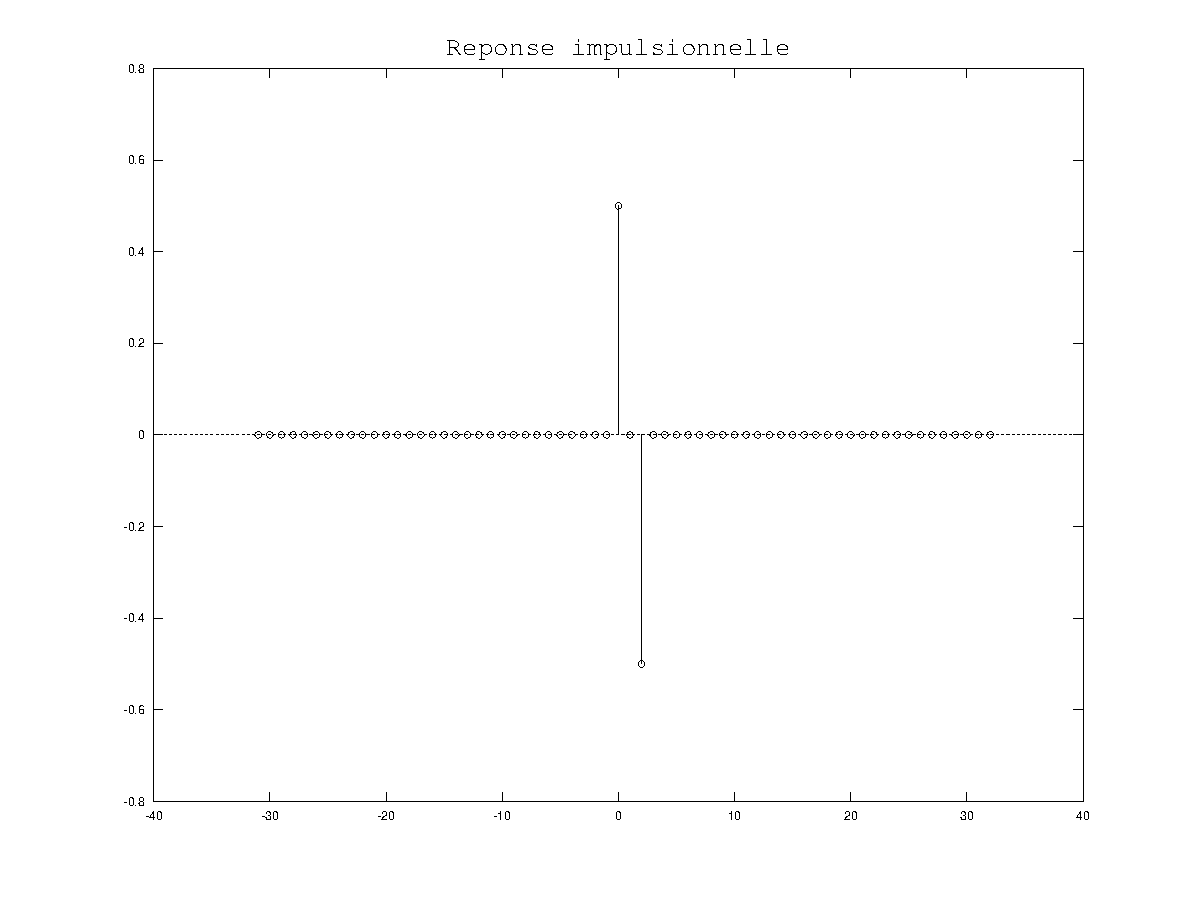
\includegraphics[width=9cm]{resEx3/f3Impulsion.pdf}
\caption{Réponse impulsionnelle de la fonction $\frac{1-z^{-2}}{2}$ }
\end{figure}

\subsection{Réponse indicielle}
~\\
\begin{figure}[H]
\centering
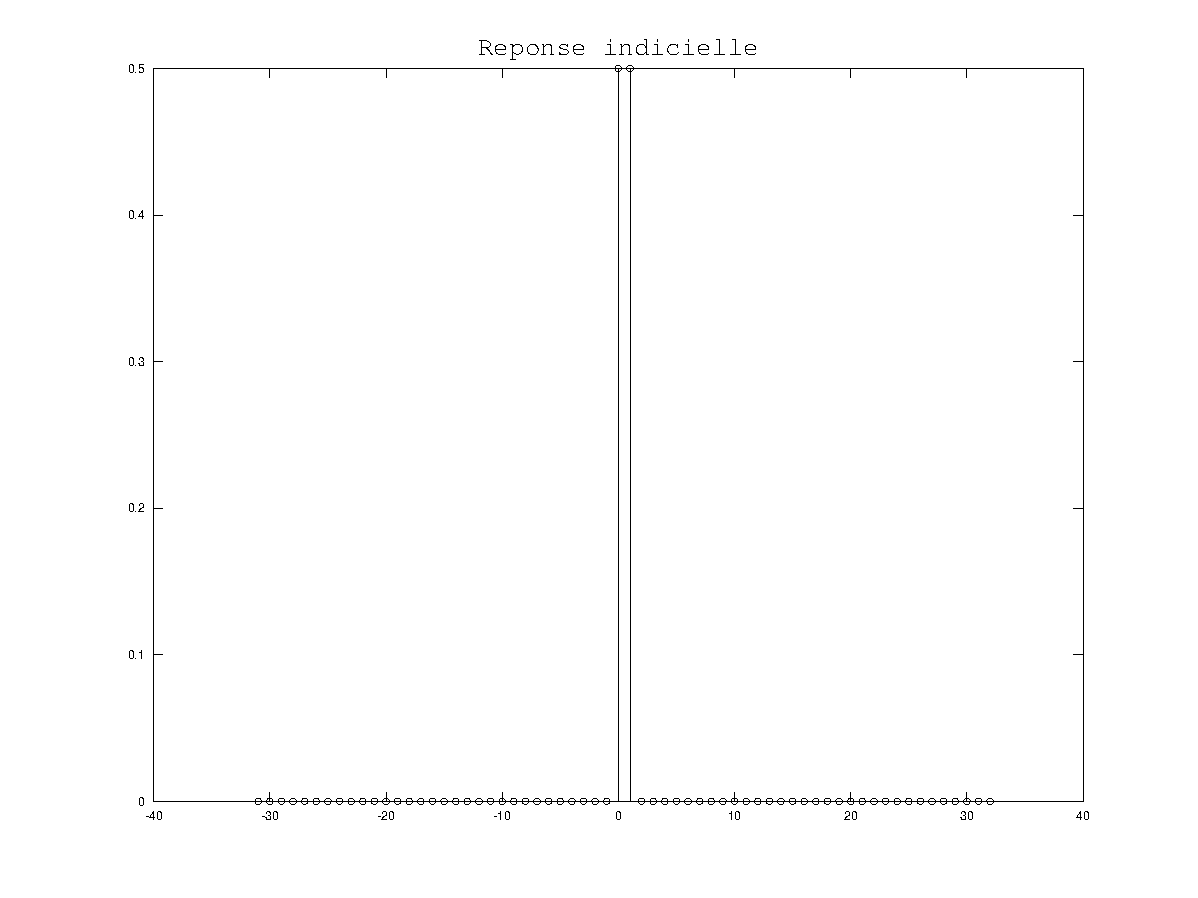
\includegraphics[width=9cm]{resEx3/f3Indice.pdf}
\caption{Réponse indicielle de la fonction $\frac{1-z^{-2}}{2}$ }
\end{figure}

\subsection{Les zéros et les pôles}
~\\
\begin{figure}[H]
\centering
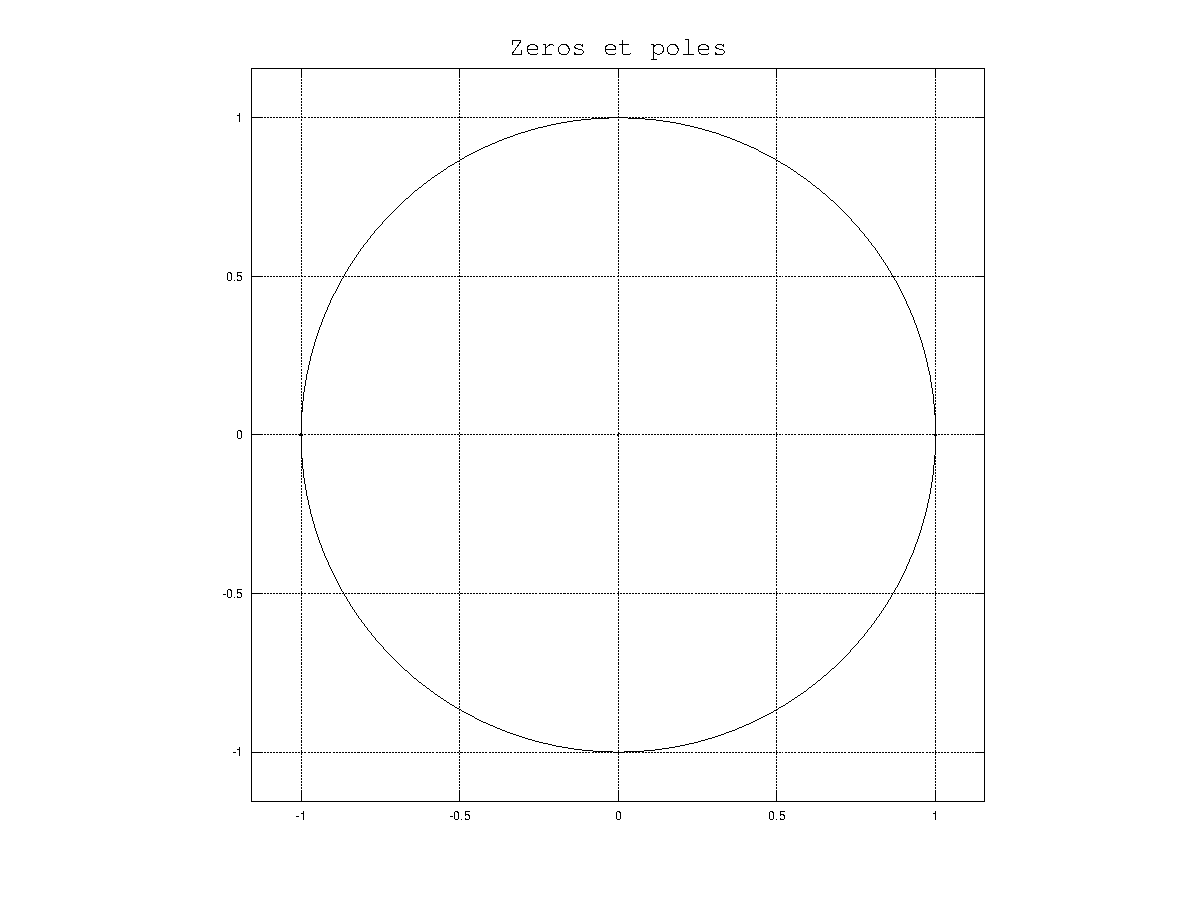
\includegraphics[width=9cm]{resEx3/f3ZP.pdf}
\caption{Les zéros et les pôles de la fonction $\frac{1-z^{-2}}{2}$ }
\end{figure}


\section{Fonction $\frac{2z^{-1}}{2-z^{-1}}$}
Nous commençons par afficher le diagramme de gain en décibel (\ref{f4 Diagramme de gain}) ainsi que le diagramme de phase en radians (\ref{f4 Diagramme de phase}) pour déterminer la nature du filtre représenté par cette fonction de transfert.
\begin{figure}[H]
\centering
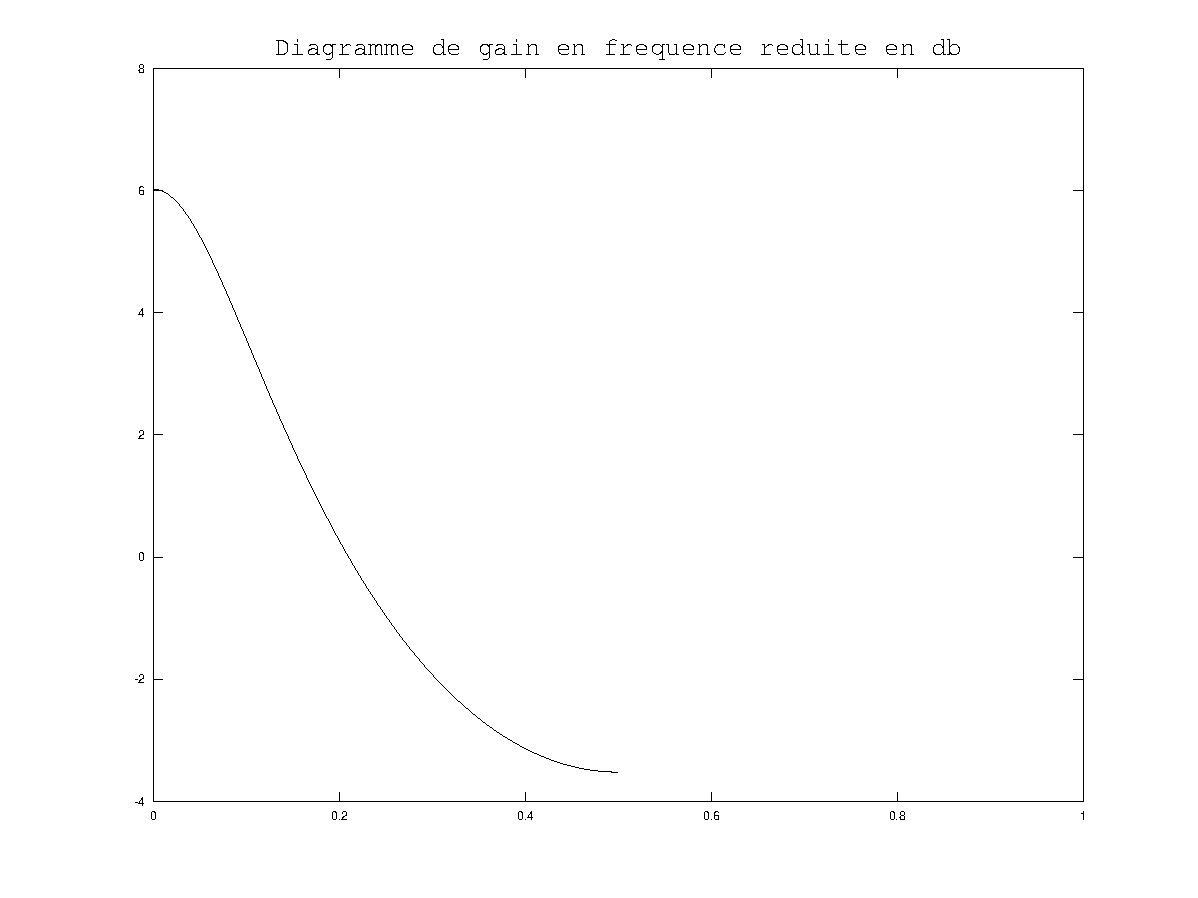
\includegraphics[width=9cm]{resEx3/f4Gain.pdf}
\caption{Diagramme de gain de la fonction $\frac{2z^{-1}}{2-z^{-1}}$ en dB}
\label{f4 Diagramme de gain}
\end{figure}
\begin{figure}[H]
\centering
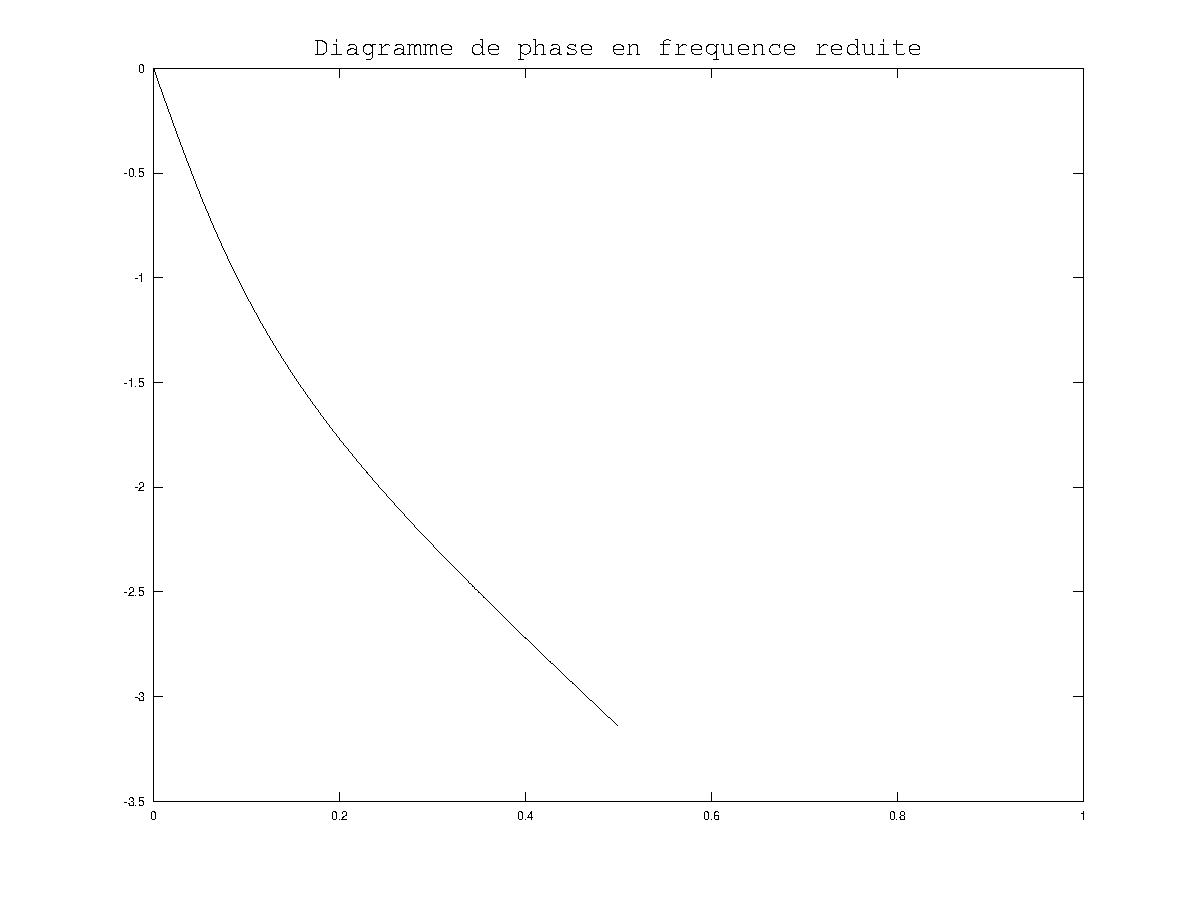
\includegraphics[width=9cm]{resEx3/f4Phase.pdf}
\caption{Diagramme de phase de la fonction $\frac{2z^{-1}}{2-z^{-1}}$ en radians}
\label{f4 Diagramme de phase}
\end{figure}
Nous pouvons donc constater que cette fonction de transfert en z correspond à un filtre passe bas.
\subsection{Réponse impulsionnelle}
~\\
\begin{figure}[H]
\centering
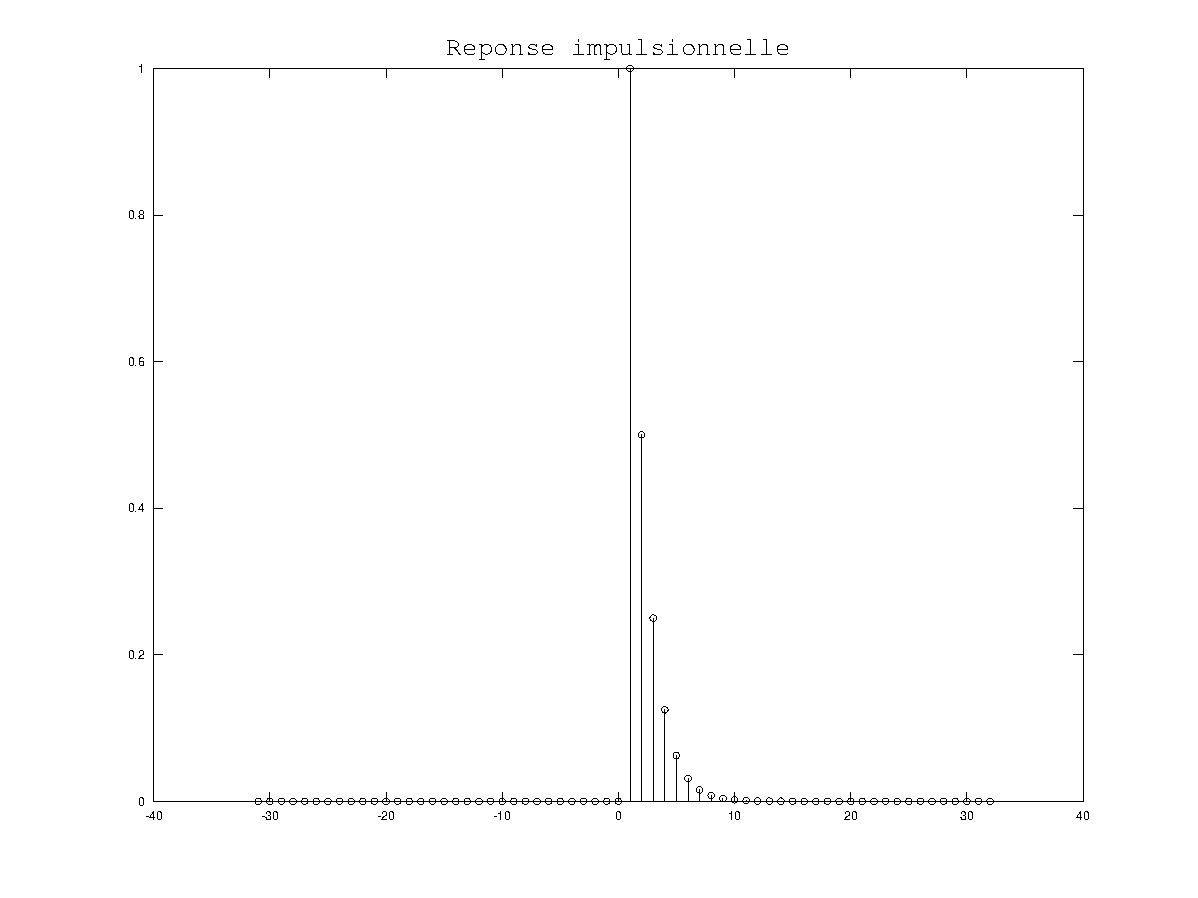
\includegraphics[width=9cm]{resEx3/f4Impulsion.pdf}
\caption{Réponse impulsionnelle de la fonction $\frac{2z^{-1}}{2-z^{-1}}$}
\end{figure}

\subsection{Réponse indicielle}
~\\
\begin{figure}[H]
\centering
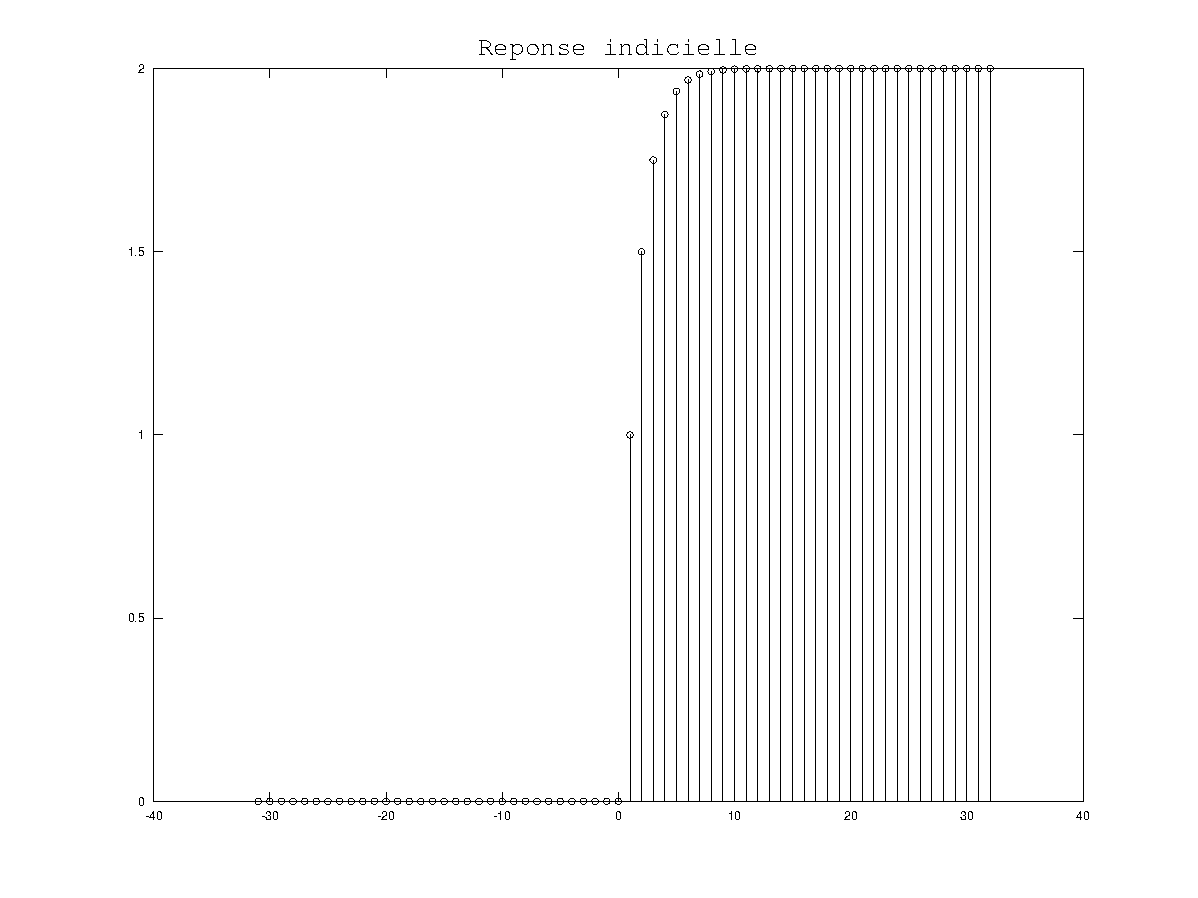
\includegraphics[width=9cm]{resEx3/f4Indice.pdf}
\caption{Réponse indicielle de la fonction $\frac{2z^{-1}}{2-z^{-1}}$}
\end{figure}

\subsection{Les zéros et les pôles}
~\\
\begin{figure}[H]
\centering
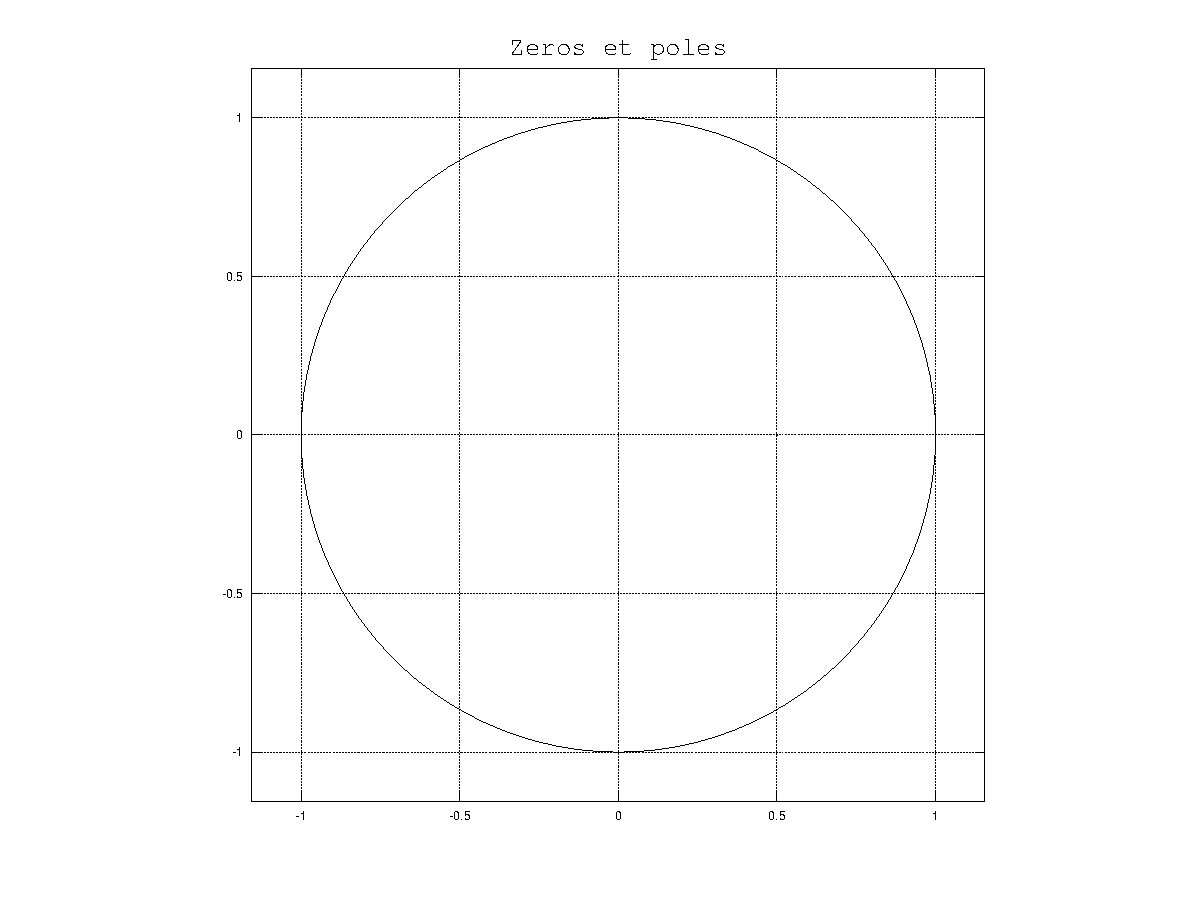
\includegraphics[width=9cm]{resEx3/f4ZP.pdf}
\caption{Les zéros et les pôles de la fonction $\frac{2z^{-1}}{2-z^{-1}}$ }
\end{figure}


\section{Fonction $\frac{2z^{-1}-z^{-5}}{2-z^{-1}}$}
Nous commençons par afficher le diagramme de gain en décibel (\ref{f5 Diagramme de gain}) ainsi que le diagramme de phase en radians (\ref{f5 Diagramme de phase}) pour déterminer la nature du filtre représenté par cette fonction de transfert.
\begin{figure}[H]
\centering
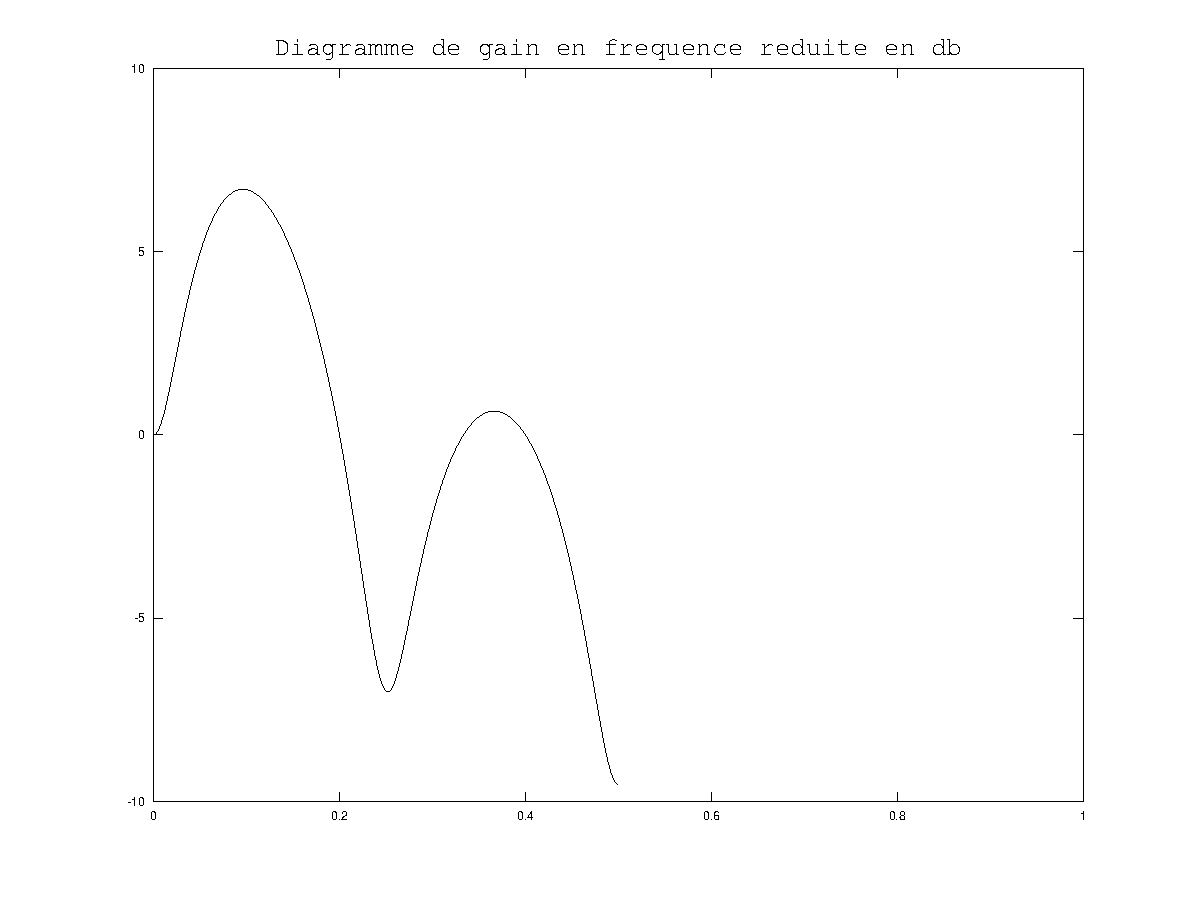
\includegraphics[width=9cm]{resEx3/f5Gain.pdf}
\caption{Diagramme de gain de la fonction $\frac{2z^{-1}-z^{-5}}{2-z^{-1}}$ en dB}
\label{f5 Diagramme de gain}
\end{figure}
\begin{figure}[H]
\centering
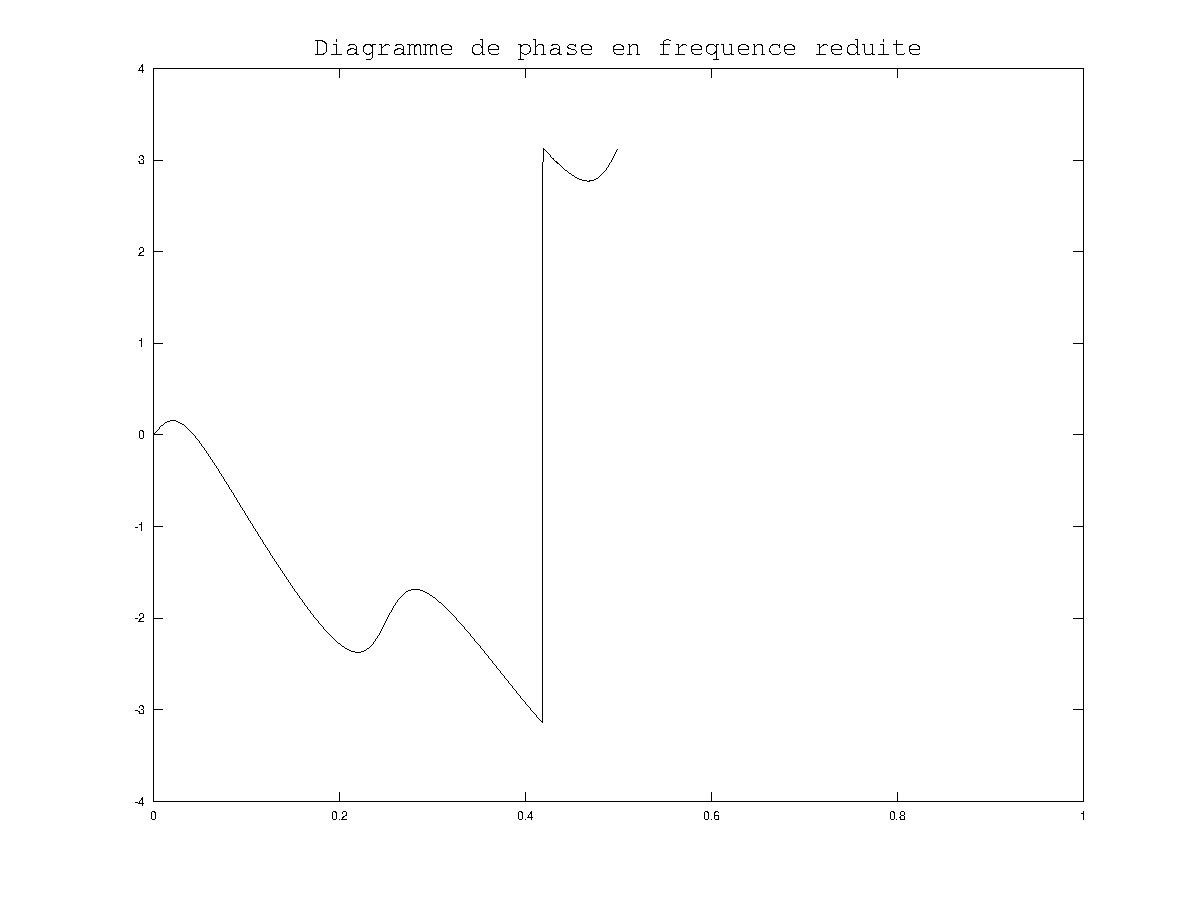
\includegraphics[width=9cm]{resEx3/f5Phase.pdf}
\caption{Diagramme de phase de la fonction $\frac{2z^{-1}-z^{-5}}{2-z^{-1}}$ en radians}
\label{f5 Diagramme de phase}
\end{figure}
Nous pouvons donc constater que cette fonction de transfert en z correspond à un filtre coupe bande.
\subsection{Réponse impulsionnelle}
~\\
\begin{figure}[H]
\centering
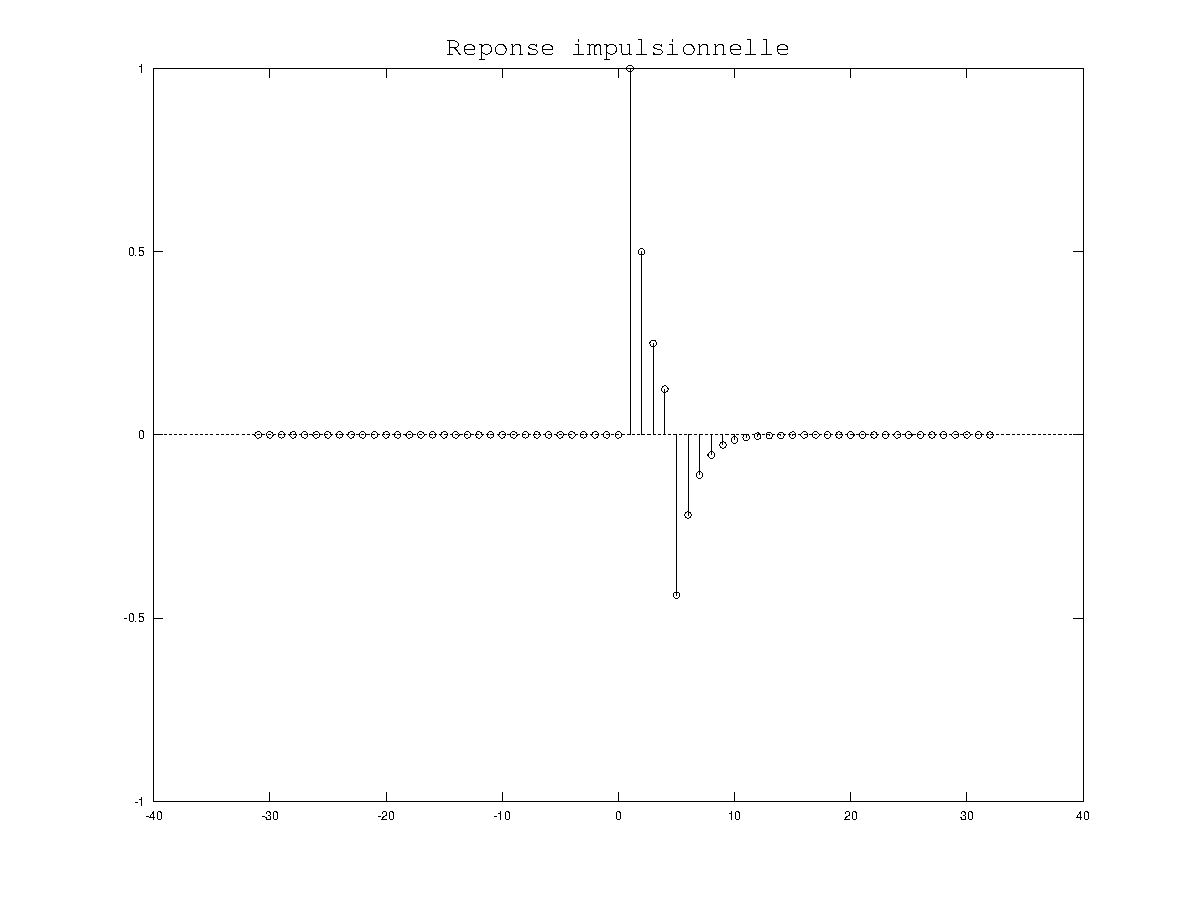
\includegraphics[width=9cm]{resEx3/f5Impulsion.pdf}
\caption{Réponse impulsionnelle de la fonction $\frac{2z^{-1}-z^{-5}}{2-z^{-1}}$ }
\end{figure}

\subsection{Réponse indicielle}
~\\
\begin{figure}[H]
\centering
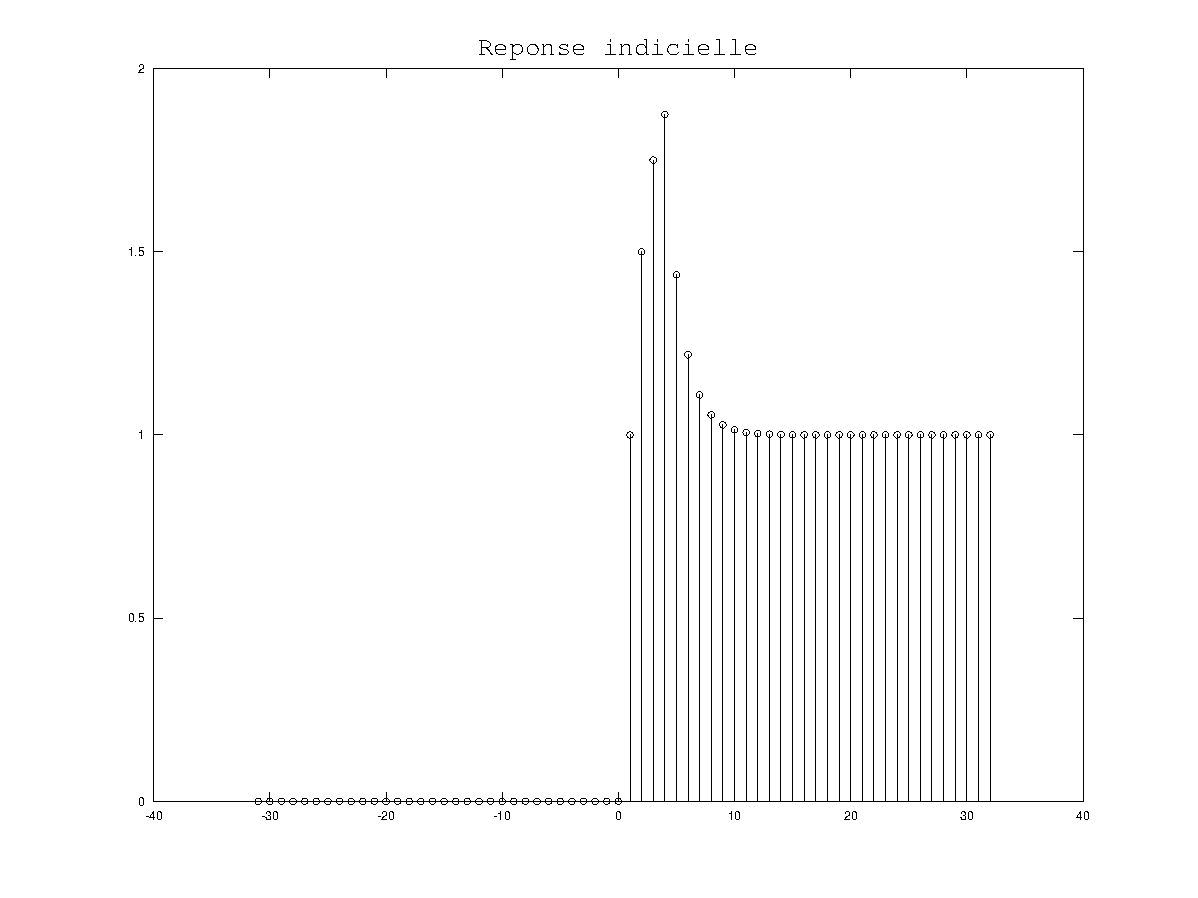
\includegraphics[width=9cm]{resEx3/f5Indice.pdf}
\caption{Réponse indicielle de la fonction $\frac{2z^{-1}-z^{-5}}{2-z^{-1}}$ }
\end{figure}

\subsection{Les zéros et les pôles}
~\\
\begin{figure}[H]
\centering
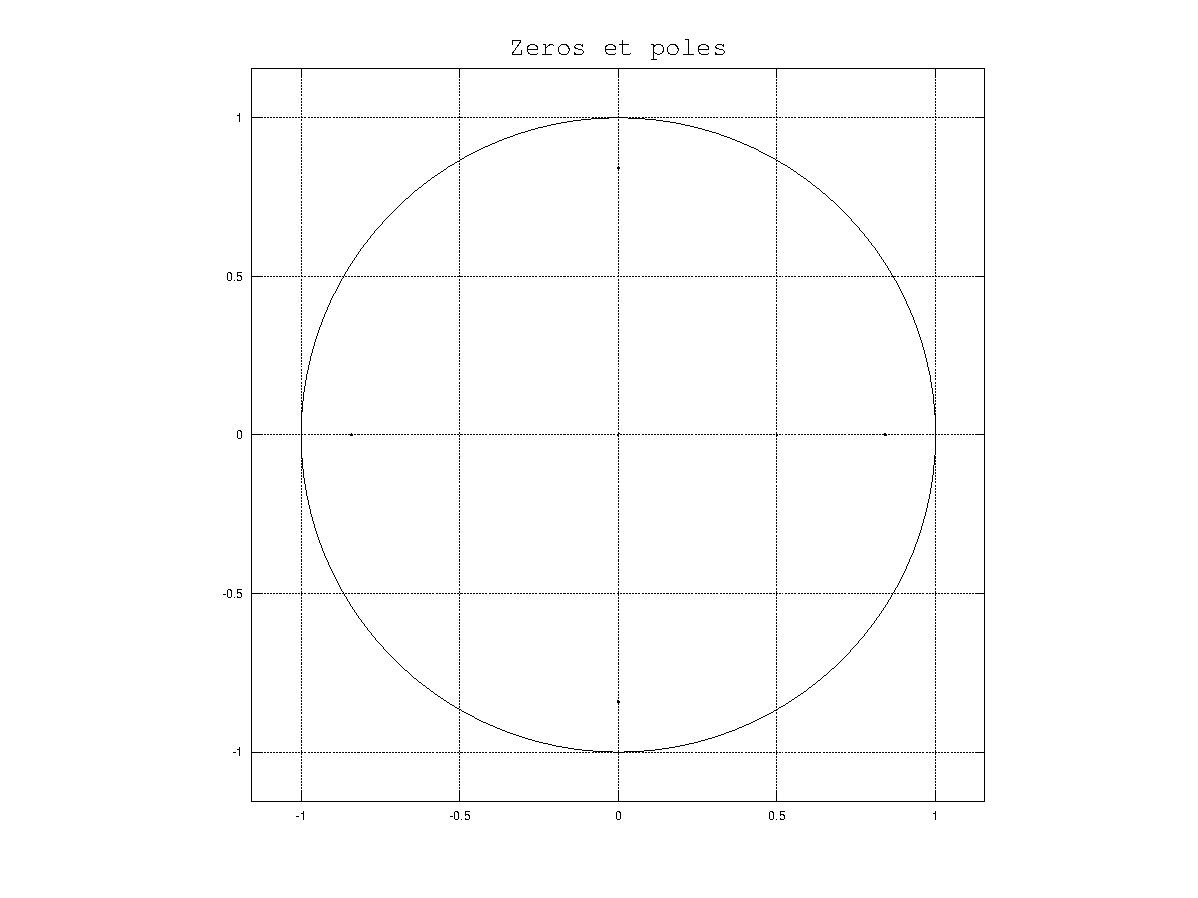
\includegraphics[width=9cm]{resEx3/f5ZP.pdf}
\caption{Les zéros et les pôles de la fonction $\frac{2z^{-1}-z^{-5}}{2-z^{-1}}$ }
\end{figure}

